\section{Web Semântica e Ontologia}

    Como apresentado até aqui, é necessário que sejam propostas novas soluções como forma de organizar os critérios de encaminhamento e priorização dos serviços básicos aos especializados. Mais que isso, possibilitar que o ordenamento e a gestão das listas de espera não fiquem refém de todos os fatores humanos associados a esse tipo de ação. Dessa forma, as tecnologias da Web Semântica podem auxiliar na gestão dessas listas, principalmente com a organização do conhecimento com as ontologias.
    
    Estima-se que na WEB existam cerca de 30 bilhões de documentos \cite{calderon2017deep}, que estão em diferentes formatos, como HTML, XML, PDF, CSV entre outros. Esses documentos são estruturados de diferentes formas para humanos, que tem a capacidade de interpretar os dados independente do formato do documento. Porém, essa diversidade de documentos acaba sendo um  grande obstáculo para o acesso, processamento e uso computacional desses dados.
    
    Em 2001, \citeonline{Berners2001} propuseram a Web Semântica, como forma de estruturar o conteúdo da web e permitir que o usuário possa realizar tarefas guiado por mecanismos chamados de agentes. Isso seria possível através da estruturação dos dados e da semântica presente em cada documento onde esses agentes virtuais conseguissem 'compreender'. Outro ganho que a proposta traria é de que as informações estariam interligadas e com fácil acesso, sendo dados interoperáveis.
    No mesmo texto de apresentação da Web Semântica publicado na revista Scientific American, os autores relatam que a Web Semântica não é uma Web separada, mas uma extensão da atual, na qual a informação recebe um significado bem definido, permitindo que computadores e pessoas trabalharem em cooperação.
    
   Para tornar a proposta aplicável, foi definida um arquitetura baseada em camadas, que pode ser melhor compreendida através da Figura 4.
   
     \begin{figure}[htb]
    	\centering
        \caption{Arquitetura da Web Semântica.}
    	\label{fig:semanticcake}
        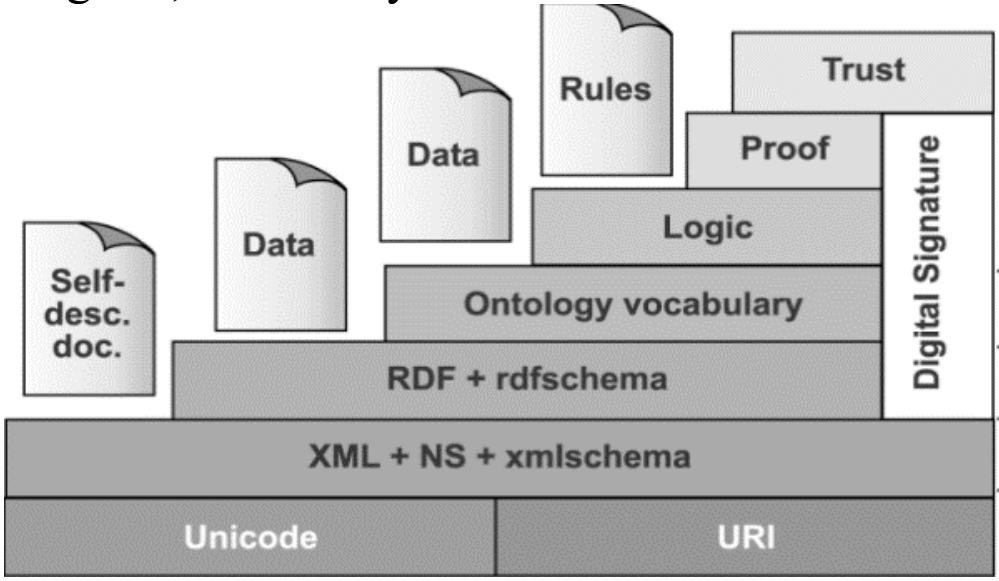
\includegraphics[width=0.7\linewidth]{images/semantic-cake}
        \fdireta{Greenberg2003}
    \end{figure}
    
    Cada camada do chamado "bolo de noiva" da web semântica foi definida com o intuito de atingir o objetivo do modelo proposto.
    
    \begin{itemize}
    	\item \textit{Unicode}: é usado para representar qualquer caractere de maneira única, seja qual for o caractere e o idioma  que ele tenha sido escrito;
        \item \sigla{URI}{\textit{Uniform Resource Identifier}}: é uma representação única de um recurso;
        \item \sigla{XML}{\textit{eXtensible Markup Language}}: é uma linguagem de marcação e representação sintática de recursos de  maneira independente de plataforma a fim de agregar semântica aos documentos;
        \item \sigla{RDF}{\textit{Resource Description Framework}}: é um modelo padrão para intercâmbio de dados. Possui recursos que facilitam a mesclagem de dados, mesmo se os esquemas subjacentes forem diferentes, e suporta especificamente a evolução dos esquemas ao longo do tempo, sem exigir que todos os consumidores de dados sejam alterados;
        \item \textit{Ontology}: coleção de termos usados para descrever um domínio através das relações e classificações desses termos;
        \item \textit{Logic}: permite a definição de regras lógicas para deduzir e inferir novas informações. Essas regras são capazes de alterar dinamicamente a estrutura da ontologia;
        \item \textit{Proof}: provê mecanismos para averiguar a confiabilidade das fontes de informações;
        \item \textit{Trust}: representa o conhecimento validado e confiável;
        \textit{Digital Signature}: permite a integração de métodos de segurança que garantam a segurança da informação.
    \end{itemize}
    
    As ontologias exercem um papel fundamental na Web Semântica, pois são elas que permitem a relação de termos e conceitos de um domínio.
    
    \subsection{Ontologias}
    
        O termo ontologia pode ter mais de um significado, dependendo da área de conhecimento onde for utilizado. Seu surgimento se deu na filosofia, sendo uma teoria sobre a natureza da existência e envolve uma categorização muito ampla da realidade \cite{CHATEUABRIAND1998}.
        
        Ontologia na ciência da computação começou a ser utilizada no início dos anos 90, para organização de grandes bases de conhecimento, seu uso se dava para a construção de grandes bases interoperáveis e melhor estruturadas \cite{MOREIRA2004}. 
        
        Na Web Semântica, as ontologias são usadas para descrever os conceitos de um domínio e a relação entre eles. O W3C relata que as ontologias devem prover descrições para os seguintes tipos de conceitos \cite{breitman2005web}:
        
        \begin{itemize}
    	\item  Classes (ou coisas) nos vários domínios de interesse;
        \item  Relacionamento entre as classes;
        \item  Propriedades (ou atributos) que as classes podem ter; 
        \end{itemize}
        
   
	\subsection{\textit{Resource Description Framework} e \textit{Web Ontology Language}}
    
    	O RDF pode ser definido como um modelo padrão para intercâmbio de dados na Web. Ele é muito utilizado por conta de suas características que facilitam a fusão de dados, além de suportar a evolução dos esquemas sem a necessidade de que todos os dados sejam alterados, referenciando a relação de diferentes recursos \cite{W3C2014}.
    	Esse framework foi desenvolvido para descrever recursos na Web. Segundo \citeonline{Shadbolt2006}, o objetivo do RDF é prover uma representação minimalista do conhecimento da Web.
    	A estrutura do RDF é formada por triplas (Sujeito, Predicado, Objeto), como pode ser visto na Figura 5, sendo:
    	
        \begin{itemize}
        	\item Sujeito: recursos  identificados por URIs;
            \item Predicado: atributos ou relações que descrevem o sujeito e o relaciona a um objeto;
            \item Objeto: um outro recurso ou valor que se relaciona com o sujeito através do predicado;
        \end{itemize}
        
         \begin{figure}[htbp]
        	\centering
            \caption{Exemplo de grafo}
            \label{fig:owl2-profiles}
            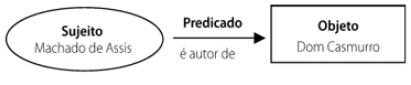
\includegraphics[width=0.7\linewidth]{images/exemplo-tripla.png}
            \fdireta{SANTOSNETO2013}
        \end{figure}
    	
    	Através das triplas é possível representar o conhecimento de qualquer domínio. No caso da área da saúde, um exemplo de representação seria: uma pessoa, suas propriedades(idade, nome, sexo) e as possíveis relações que essa pessoa pode ter (doenças que teve, medicações aplicadas, exames realizados). 
        
        Como dito anteriormente, o RDF é um framework para descrever recursos, mas em qual formato? Qual estrutura? RDF pode ser serializado para diferentes formatos de acordo com a necessidade do uso. Na Figura 6 são apresentados os formatos de serialização do RDF, bem como a estrutura do código para cada formato e o propósito de uso de cada um.
         
         \begin{figure}[htbp]
        	\centering
            \caption{Formatos de serialização RDF}
            \label{fig:owl2-profiles}
            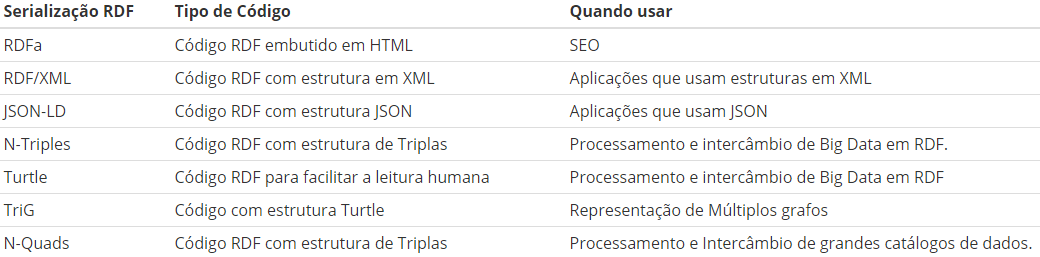
\includegraphics[width=1\linewidth]{images/serializacoes-rdf.png}
            \fdireta{isotani2015dados}
        \end{figure}
        
        Apesar do RDF permitir a descrição de ontologias, há algumas limitações quanto ao nível de expressividade que é possível alcançar, por consequência poucas inferências (capacidade que o computador deduza informações através de declarações estabelecidas) são possíveis. Por isso, foi desenvolvida uma linguagem mais expressiva denominada Web Ontology Language (OWL).
        
        A OWL também foi desenvolvida e é recomendada pelo W3C. Essa linguagem tem uma expressividade maior que o RDF ampliando suas possibilidades de representação de conhecimento. A primeira versão da OWL (1.0), possui 3 perfis de expressividade que permitem que aplicações, com diferentes objetivos, sejam construídas. Eles formam uma família de três variantes linguísticas de crescente poder expressivo: OWL Lite, OWL DL e OWL Full \cite{isotani2015dados}.
        
        Uma das limitações importantes da OWL 1 era a falta de um conjunto adequado de tipos de dados internos. Isso porque OWL depende do esquema XML (xsd) para a lista de tipos de dados internos. Por isso, uma nova versão foi criada: a OWL 2. Essa versão melhora consideravelmente os tipos de dados, além de abordar problemas agudos com expressividade. Um objetivo no desenvolvimento do OWL 2 foi fornecer uma plataforma robusta para o desenvolvimento futuro. Na OWL 2 foram definidos cinco perfis diferentes que podem ser utilizados para fins de representação distintos, são eles:
        
        \begin{itemize}
        	\item Full: o nível mais completo de expressividade de OWL, porém não tem a garantia de decidibilidade computacional;
            \item DL: possui o máximo de expressividade e a garantia computacional de que todas as inferências são computáveis e que têm decidibilidade com as inferências terminando em tempo finito;
            \item EL: adequada para ontologias que definem um grande número de classes e/ou propriedades;
            \item QL: possibilita a inferência em ontologias menos complexas e que possuem dados mais estruturados, como banco de dados relacionais.
            \item RL: é voltado para aplicativos que exigem raciocínio escalável sem sacrificar muita energia com expressividade. Ele é projetado para acomodar aplicativos OWL 2 que podem trocar a expressividade total da linguagem pela eficiência.
        \end{itemize}